\documentclass[12pt,UTF8]{ctexart}
\usepackage{ctex,amsmath,amssymb,geometry,fancyhdr,bm,amsfonts,mathtools,extarrows,graphicx,url,enumerate,xcolor,float,multicol,wasysym}
\usepackage{subfigure}

\allowdisplaybreaks[4]
% 加入中文支持
\newcommand\Set[2]{\left\{#1\ \middle\vert\ #2 \right\}}
\newcommand\Lim[0]{\lim\limits_{n\rightarrow\infty}}
\newcommand\LIM[2]{\lim\limits_{#1\rightarrow#2}}
\newcommand\Ser[1]{\sum_{n=#1}^\infty}
\newcommand{\SER}[2]{\sum_{#1=#2}^\infty}
\newcommand{\Int}[4]{\varint\nolimits_{#1}^{#2}#3\mathrm d#4}
\newcommand{\aIInt}[1]{\iint\limits_{#1}}
\newcommand{\IInt}[3]{\iint\limits_{#1}#2\mathrm d#3}
\newcommand{\varIInt}[4]{\iint\limits_{#1}#2\mathrm d#3\mathrm d#4}
\newcommand{\IIInt}[3]{\iiint\limits_{#1}#2\mathrm d#3}
\newcommand{\varIIInt}[5]{\iiint\limits_{#1}#2\mathrm d#3\mathrm d#4\mathrm d#5}
\newcommand{\LInt}[3]{\varint\nolimits_{#1}#2\mathrm d#3}
\newcommand{\LOInt}[3]{\varoint\nolimits_{#1}#2\mathrm d#3}
\newcommand{\LLInt}[4]{\varint\nolimits_{#1}\nolimits^{#2}#3\mathrm d#4}
\newcommand{\BLInt}[2]{\varint\nolimits_{#1}#2}
\newcommand{\varBLInt}[3]{\varint\nolimits_{#1}\nolimits^{#2}#3}
\newcommand{\BLOInt}[2]{\varoint\nolimits_{#1}#2}
\newcommand{\SIInt}[3]{\iint\limits_{#1}#2\mathrm d#3}
\newcommand{\md}[1]{\mathrm d#1}
\newcommand{\BSIInt}[2]{\iint\limits_{#1}#2}
\newcommand{\pp}[2]{\frac{\partial #1}{\partial #2}}
\newcommand{\ppx}[1]{\frac{\partial #1}{\partial x}}
\newcommand{\ppy}[1]{\frac{\partial #1}{\partial y}}
\newcommand{\ppz}[1]{\frac{\partial #1}{\partial z}}
\newcommand{\varppx}[1]{\frac{\partial}{\partial x} #1}
\newcommand{\varppy}[1]{\frac{\partial}{\partial y} #1}
\newcommand{\varppz}[1]{\frac{\partial}{\partial z} #1}
\newcommand{\BSOIInt}[2]{\oiint\limits_{#1}#2}
\newcommand{\me}[0]{\mathrm e}
\newcommand{\m}[0]{\mathrm }
\newcommand{\dd}[2]{\frac{\mathrm d #1}{\mathrm d #2}}
\geometry{a4paper,scale=0.80}
\pagestyle{fancy}
\rhead{习题14.5}
\lhead{基础习题课讲义}
\chead{微积分B(2)}
\begin{document}
\setcounter{section}{27}
\section{线性常微分方程组}
\subsection{知识结构}
\noindent第14章 常微分方程
	\begin{enumerate}
		\item[14.5]线性微分方程组
			\begin{enumerate}
				\item[14.5.1]一般理论
				\item[14.5.2]线性微分方程组解的结构
				\item[14.5.3]常系数微分方程组的解
			\end{enumerate}
	\end{enumerate}
\subsection{线性微分方程组}
\begin{figure}[H]
\begin{center}
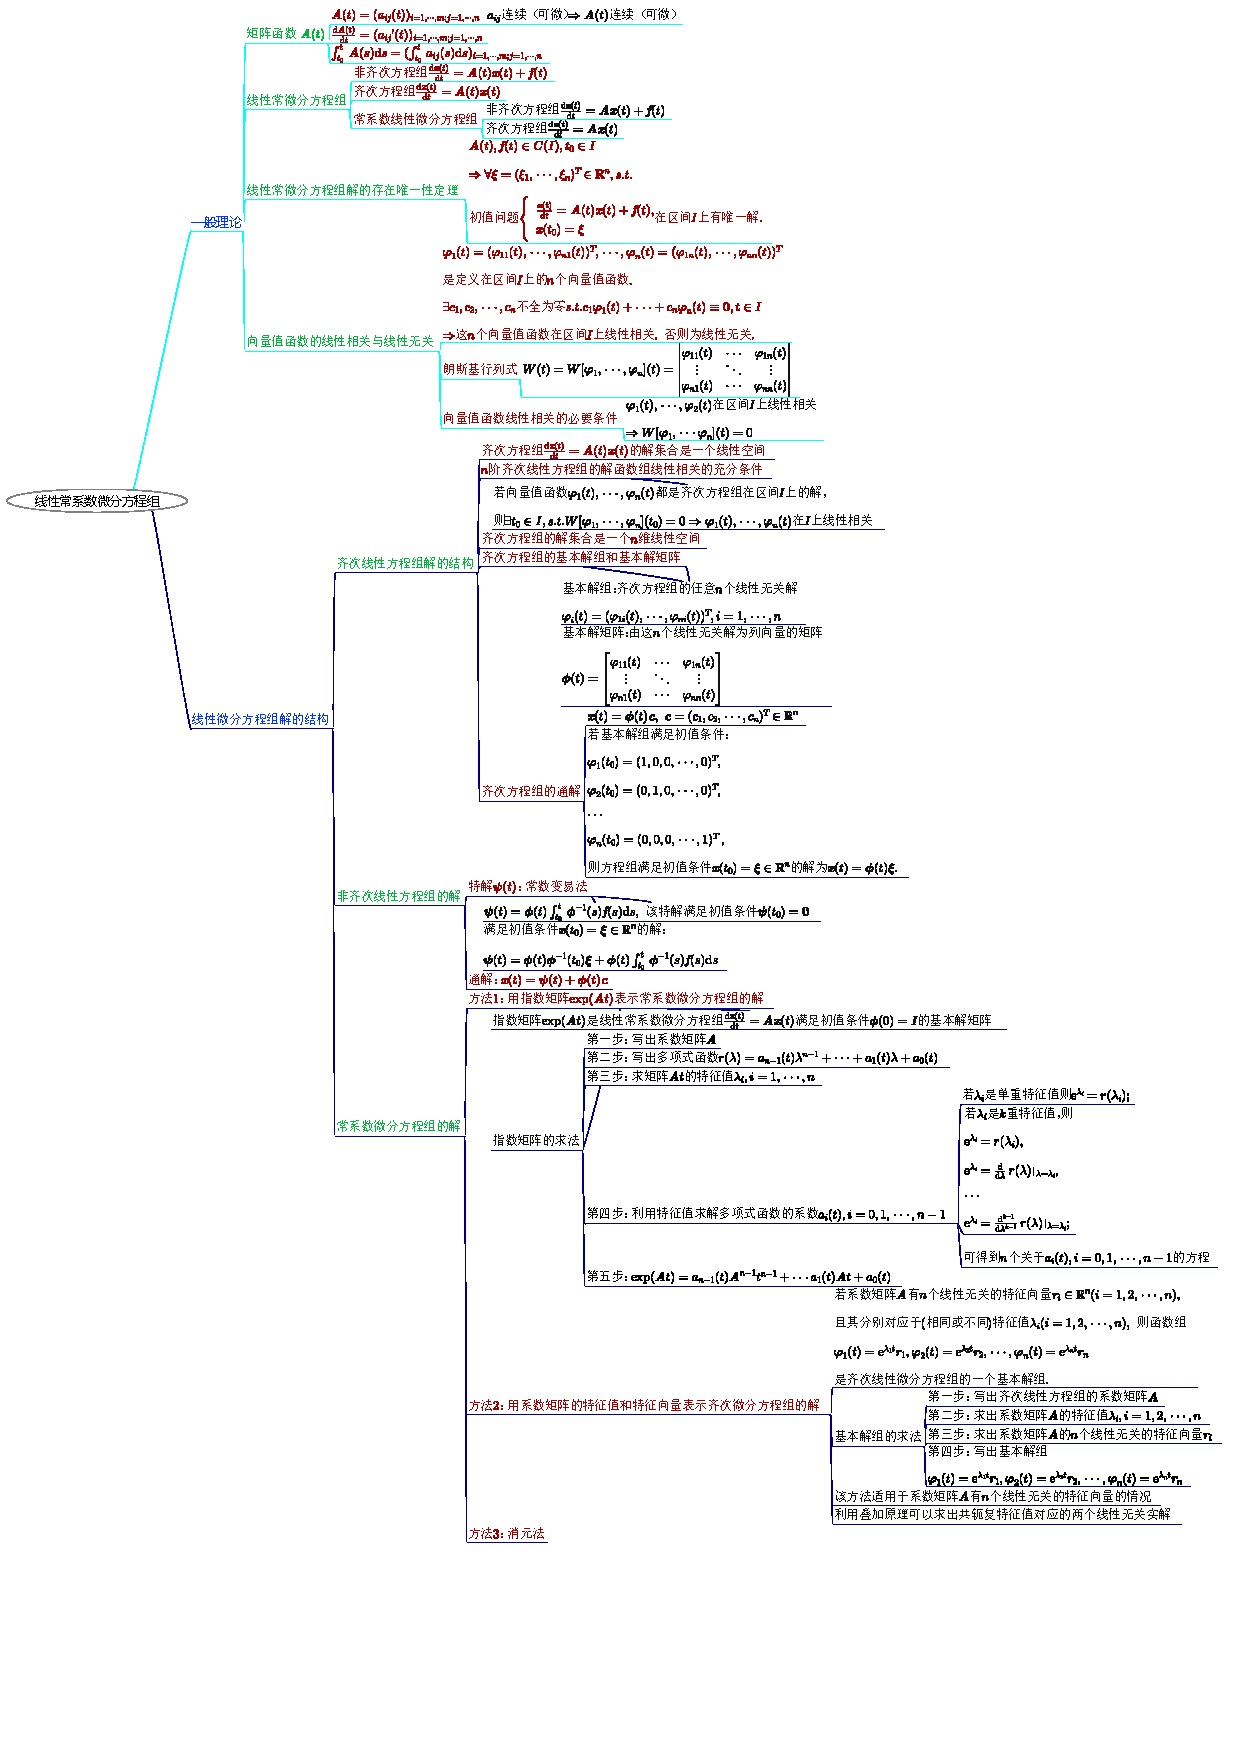
\includegraphics[height=1\textheight]{Figures28/Structures.pdf}
\end{center}
\end{figure}
\subsection{齐次线性常系数微分方程组的解法}\label{homo-lin-eq}
\begin{enumerate}
\item方法1:用指数矩阵$\exp(\bm At)$表示线性常系数微分方程组的解. 指数矩阵$\exp(\bm At)$是线性常系数微分方程组$\dd{\bm x(t)}t=\bm A\bm x(t)$的基本解矩阵,其求法可参考以下步骤:
\begin{enumerate}
\item[第一步]写出齐次线性方程组的系数矩阵$\bm A$;
\item[第二步]写出多项式函数$r(\lambda)=a_{n-1}(t)\lambda^{n-1}+\cdots+a_1(t)\lambda+a_0$;
\item[第三步]求矩阵$\bm At$的特征值$\lambda_i,i=1,2,\cdots,n$;
\item[第四步]利用特征值求解多项式函数$r(\lambda)$的系数$a_i(t),i=1,2,\cdots,n$:
\begin{enumerate}
\item[(1)]对于单重特征值$\lambda_i,a_i(t)$满足$\me^{\lambda_i}=r(\lambda_i)$;
\item[(2)]对于$k$重特征值$\lambda_i,a_i(t)$满足$\begin{cases}
\me^{\lambda_i}=r(\lambda_i),\\
\me^{\lambda_i}=\dd{r(\lambda)}\lambda\big|_{\lambda=\lambda_i},\\
\cdots\\
\me^{\lambda_i}=\dd{r^{k-1}(\lambda)}{\lambda^{k-1}}\big|_{\lambda=\lambda_i}.
\end{cases}$
\item[(3)]可据此得到$n$个关于$a_i(t)$的方程,从而求出$a_i(t),i=1,2,\cdots,n$.
\end{enumerate}
\item[第五步]基本解矩阵
\[\exp(\bm At)=a_{n-1}(t)\bm A^{n-1}t^{n-1}+\cdots+a_1(t)\bm At+a_0t.\]
\end{enumerate}
\item方法2:用系数矩阵的特征值和特征向量表示线性常系数微分方程组的解. 若系数矩阵有$n$个线性无关的特征向量$\bm r_i\in\mathbb R^n(i=1,2,\cdots,n)$, 且其分别对应于(相同或不同)特征值$\lambda_i(i=1,2,\cdots,n)$, 则函数组$\bm\varphi_1(t)=\me^{\lambda_1t}\bm r_1,\bm\varphi_2(t)=\me^{\lambda_2t}\bm r_2,\cdots,\bm\varphi_i(t)=\me^{\lambda_nt}\bm r_n(t)$是齐次方程组的一个基本解组. 基本解组的求法可参考以下步骤:
\begin{enumerate}
\item[第一步]写出齐次线性方程组的系数矩阵$\bm A$;
\item[第二步]求出系数矩阵$\bm A$的特征值$\lambda_i,i=1,2,\cdots,n$;
\item[第三步]求出系数矩阵$\bm A$的$n$个线性无关的特征向量$\bm r_i,i=1,2,\cdots,n$;
\item[第四步]写出基本解组
\[\bm\varphi_1(t)=\me^{\lambda_1t}\bm r_1,\bm\varphi_2(t)=\me^{\lambda_2t}\bm r_2,\cdots,\bm\varphi_i(t)=\me^{\lambda_nt}\bm r_n(t).\]
\end{enumerate}
{\bf注意:}
\begin{enumerate}
\item该方法适用于$k$重特征值对应有$k$个线性无关的特征向量的情况,即矩阵$\bm A$有$n$个线性无关的特征向量. 若系数矩阵$\bm A$有少于$n$个的线性无关的特征向量,则可采用上述方法1或下述方法3.

【如习题14.5中的1.(3)/(6).】
\item复特征值的情况. 设$\lambda_{\pm}=\alpha\pm\beta\m i$是系数矩阵$\bm A$的一对共轭复特征值,$\bm r_{\pm}=\bm a\pm\bm b\m i$是与其对应的特征向量,则$\begin{cases}
\me^{\lambda_+t}\bm r_+=\me^{(\alpha+\beta\m i)t}(\bm a+\bm b\m i),\\
\me^{\lambda_-t}\bm r_-=\me^{(\alpha-\beta\m i)t}(\bm a-\bm b\m i)
\end{cases}$是微分方程的两个线性无关解. 利用叠加原理知$\begin{cases}
\text{Re}(\me^{\lambda_+t}\bm r_+)=\me^{\alpha t}(\bm a\cos\beta t-\bm b\sin\beta t),\\
\text{Im}(\me^{\lambda_+t}\bm r_+)=\me^{\alpha t}(\bm b\cos\beta t+\bm a\sin\beta t)
\end{cases}$是微分方程的两个线性无关的实解.
\end{enumerate}
\item消元法. 适用于二阶齐次线性方程组

【如习题14.5中的1.(1)/(2)/(3)/(4),2.(1)/(4)】

和简单的三阶及以上的线性方程组

【如习题14.5中的2.(2)】.

具体解题步骤可参看上述习题.
\item三种方法的比较:
\begin{enumerate}
\item三种方法中消元法较简单且不易出错,如能用消元法,可直接用消元法求解. 
\item方法2相对于方法1简单且不易出错,但如果系数矩阵线性无关的特征向量的个数少于$n$则不适用.
\item方法1是一种万能的解法,但计算量较大,容易出错. 如果消元法和方法2都不适用,则可用方法1求解.
\end{enumerate}
\end{enumerate}
\subsection{非齐次线性常系数微分方程组的解法}
非齐次线性常系数微分方程组的求解可参考以下步骤:
\begin{enumerate}
\item[第一步]用\ref{homo-lin-eq}中的方法求解该非齐次方程组对应的齐次方程组的基本解矩阵$\bm\phi(t)$;
\item[第二步]求$\bm\phi^{-1}(t)$;
\item[第三步]代入公式$\bm x(t)=\bm\phi(t)\bm c+\bm\phi(t)\Int{t_0}t{\bm\phi^{-1}(t)\bm  f(t)}t$求解非齐次线性方程组的通解. 若已知初值条件$\bm x(t_0)=\bm\xi$,则可代入公式$\bm x(t)=\bm\phi(t)\bm\phi^{-1}(t_0)\bm\xi+\bm\phi(t)\Int{t_0}t{\bm\phi^{-1}(t)\bm  f(t)}t$求解非齐次线性方程组的通解.
\end{enumerate}
\subsection{习题14.5解答}
\begin{enumerate}
\item求下列方程组满足指定条件的解:\\
(1)$\begin{cases}
\dd{x_1}t=x_1+x_2,\\
\dd{x_2}t=2x_1-4x_2,
\end{cases}(x_1(0),x_2(0))=(1,-1)$;\\
(2)$\begin{cases}
\dd{x_1}t=x_1+2x_2,\\
\dd{x_2}t=4x_1+3x_2,
\end{cases}(x_1(0),x_2(0))=(1,0)$;\\
(3)$\begin{cases}
\dd{x_1}t=x_1-x_2,\\
\dd{x_2}t=x_1+3x_2,
\end{cases}(x_1(0),x_2(0))=(2,3)$;\\
(4)$\begin{cases}
\dd{x_1}t=4x_1-2x_2,\\
\dd{x_2}t=x_1-4x_2,
\end{cases}(x_1(0),x_2(0))=(1,0)$;\\
(5)$\begin{cases}
\dd{x_1}t=x_2+x_3,\\
\dd{x_2}t=x_3+x_1,\\
\dd{x_3}t=x_1+x_2,
\end{cases}(x_1(0),x_2(0),x_3(0))=(2,3,1)$;\\
(6)$\begin{cases}
\dd{x_1}t=x_2-x_1,\\
\dd{x_2}t=4x_3-x_2,\\
\dd{x_3}t=x_1-4x_3,
\end{cases}(x_1(0),x_2(0),x_3(0))=(2,3,1)$.

解:(1)方法1:方程组的系数矩阵为$\bm A=\begin{bmatrix}1&1\\2&-4\end{bmatrix}$,

\[\exp(\bm At)=a_1\bm At+a_0\bm I=\begin{bmatrix}a_1t+a_0&a_1t\\2a_1t&-4a_1t+a_0\end{bmatrix},\ r(\lambda t)=a_1\lambda t+a_0,\]

由$\det(\lambda I-A)=\begin{vmatrix}\lambda-1&-1\\-2&\lambda+4\end{vmatrix}=(\lambda-1)(\lambda+4)-2=\lambda^2+3\lambda-6=0$得特征值$\lambda_{1,2}=\frac{-3\pm\sqrt{9+4\times6}}2=\frac{-3\pm\sqrt{33}}2$, 则$a_1,a_0$满足
\[\me^{\frac{-3-\sqrt{33}}2t}=a_1\cdot(\frac{-3-\sqrt{33}}2t)+a_0,\ \me^{\frac{-3+\sqrt{33}}2t}=a_1\cdot(\frac{-3+\sqrt{33}}2t)+a_0,\]
则
\[\begin{aligned}
a_1&=\frac{\me^{\frac{-3+\sqrt{33}}2t}-\me^{\frac{-3-\sqrt{33}}2t}}{\sqrt{33}t},\\
a_0&=\frac{\me^{\frac{-3+\sqrt{33}}2t}+\me^{\frac{-3-\sqrt{33}}2t}}2+\frac32t\frac{\me^{\frac{-3+\sqrt{33}}2t}-\me^{\frac{-3-\sqrt{33}}2t}}{\sqrt{33}t}\\
&=\frac12(1+\frac3{\sqrt{33}})\me^{\frac{-3+\sqrt{33}}2t}+\frac12(1-\frac3{\sqrt{33}})\me^{\frac{-3-\sqrt{33}}2t},
\end{aligned}\]
$\therefore$
\[\begin{aligned}
a_1t+a_0&=\frac{\me^{\frac{-3+\sqrt{33}}2t}-\me^{\frac{-3-\sqrt{33}}2t}}{\sqrt{33}t}t+\frac12(1+\frac3{\sqrt{33}})\me^{\frac{-3+\sqrt{33}}2t}+\frac12(1-\frac3{\sqrt{33}})\me^{\frac{-3-\sqrt{33}}2t}\\
&=\frac12(1+\frac5{\sqrt{33}})\me^{\frac{-3+\sqrt{33}}2t}+\frac12(1-\frac5{\sqrt{33}})\me^{\frac{-3-\sqrt{33}}2t},\\
a_1t&=\frac{\me^{\frac{-3+\sqrt{33}}2t}-\me^{\frac{-3-\sqrt{33}}2t}}{\sqrt{33}t}t=\frac1{\sqrt{33}}\me^{\frac{-3+\sqrt{33}}2t}-\frac1{\sqrt{33}}\me^{\frac{-3-\sqrt{33}}2t},\\
2a_1t&=2\frac{\me^{\frac{-3+\sqrt{33}}2t}-\me^{\frac{-3-\sqrt{33}}2t}}{\sqrt{33}t}t=\frac2{\sqrt{33}}\me^{\frac{-3+\sqrt{33}}2t}-\frac2{\sqrt{33}}\me^{\frac{-3-\sqrt{33}}2t},\\
-4a_1t+a_0&=-4\frac{\me^{\frac{-3+\sqrt{33}}2t}-\me^{\frac{-3-\sqrt{33}}2t}}{\sqrt{33}t}t+\frac12(1+\frac3{\sqrt{33}})\me^{\frac{-3+\sqrt{33}}2t}+\frac12(1-\frac3{\sqrt{33}})\me^{\frac{-3-\sqrt{33}}2t}\\
&=\frac12(1-\frac5{\sqrt{33}})\me^{\frac{-3+\sqrt{33}}2t}+\frac12(1+\frac5{\sqrt{33}})\me^{\frac{-3-\sqrt{33}}2t},
\end{aligned}\]
$\therefore$
\[
\exp(\bm At)=\begin{bmatrix}
\frac12(1+\frac5{\sqrt{33}})\me^{\frac{-3+\sqrt{33}}2t}+\frac12(1-\frac5{\sqrt{33}})\me^{\frac{-3-\sqrt{33}}2t}&\frac1{\sqrt{33}}\me^{\frac{-3+\sqrt{33}}2t}-\frac1{\sqrt{33}}\me^{\frac{-3-\sqrt{33}}2t}\\
\frac2{\sqrt{33}}\me^{\frac{-3+\sqrt{33}}2t}-\frac2{\sqrt{33}}\me^{\frac{-3-\sqrt{33}}2t}&\frac12(1-\frac5{\sqrt{33}})\me^{\frac{-3+\sqrt{33}}2t}+\frac12(1+\frac5{\sqrt{33}})\me^{\frac{-3-\sqrt{33}}2t}
\end{bmatrix},
\]
方程组的通解为
\[\bm x(t)=\exp(\bm At)\bm c,\]
$\because(x_1(0),x_2(0))=(1,-1)$,

$\therefore\bm x(0)=\exp(At)|_{t=0}\bm c=\begin{bmatrix}
1&0\\
0&1
\end{bmatrix}\begin{pmatrix}c_1\\c_2\end{pmatrix}=\begin{pmatrix}c_1\\c_2\end{pmatrix}=\begin{pmatrix}1\\-1\end{pmatrix}$,

$\therefore\bm c=\begin{pmatrix}1\\-1\end{pmatrix}$

$\therefore$满足初值条件的特解为
\[\begin{aligned}
\bm x(t)&=\begin{pmatrix}x_1(t)\\x_2(t)\end{pmatrix}=\exp(\bm At)\bm c\\
&=\begin{pmatrix}
\frac12(1+\frac5{\sqrt{33}})\me^{\frac{-3+\sqrt{33}}2t}+\frac12(1-\frac5{\sqrt{33}})\me^{\frac{-3-\sqrt{33}}2t}-[\frac1{\sqrt{33}}\me^{\frac{-3+\sqrt{33}}2t}-\frac1{\sqrt{33}}\me^{\frac{-3-\sqrt{33}}2t}]\\
\frac2{\sqrt{33}}\me^{\frac{-3+\sqrt{33}}2t}-\frac2{\sqrt{33}}\me^{\frac{-3-\sqrt{33}}2t}-[\frac12(1-\frac5{\sqrt{33}})\me^{\frac{-3+\sqrt{33}}2t}+\frac12(1+\frac5{\sqrt{33}})\me^{\frac{-3-\sqrt{33}}2t}]
\end{pmatrix}\\
&=\begin{pmatrix}
\frac12(1+\frac3{\sqrt{33}})\me^{\frac{-3+\sqrt{33}}2t}+\frac12(1-\frac3{\sqrt{33}})\me^{\frac{-3-\sqrt{33}}2t}\\
-\frac12(1-\frac9{\sqrt{33}})\me^{\frac{-3+\sqrt{33}}2t}-\frac12(1+\frac9{\sqrt{33}})\me^{\frac{-3-\sqrt{33}}2t}
\end{pmatrix}\\
&=\begin{pmatrix}
\frac12(1+\frac{\sqrt{33}}{11})\me^{\frac{-3+\sqrt{33}}2t}+\frac12(1-\frac{\sqrt{33}}{11})\me^{\frac{-3-\sqrt{33}}2t}\\
-\frac12(1-\frac{3\sqrt{33}}{11})\me^{\frac{-3+\sqrt{33}}2t}-\frac12(1+\frac{3\sqrt{33}}{11})\me^{\frac{-3-\sqrt{33}}2t}
\end{pmatrix}.
\end{aligned}\]

方法2:方程组的系数矩阵为$\bm A=\begin{bmatrix}1&1\\2&-4\end{bmatrix}$, 

由$\det(\lambda I-A)=\begin{vmatrix}\lambda-1&-1\\-2&\lambda+4\end{vmatrix}=(\lambda-1)(\lambda+4)-2=\lambda^2+3\lambda-6=0$得特征值$\lambda_{1,2}=\frac{-3\pm\sqrt{9+4\times6}}2=\frac{-3\pm\sqrt{33}}2$, 

由$(\lambda_1\bm I-\bm A)\bm r=(\frac{-3+\sqrt{33}}2\bm I-\bm A)\bm r=\begin{bmatrix}
\frac{-3+\sqrt{33}-2}2&-1\\
-2&\frac{-3+\sqrt{33}+8}2
\end{bmatrix}\bm r=\begin{bmatrix}
\frac{-5+\sqrt{33}}2&-1\\
-2&\frac{5+\sqrt{33}}2
\end{bmatrix}\bm r=\bm0=\begin{bmatrix}
\frac{33-25}4&\frac{-5-\sqrt{33}}2\\
-2&\frac{5+\sqrt{33}}2
\end{bmatrix}\bm r=\begin{bmatrix}
2&\frac{-5-\sqrt{33}}2\\
-2&\frac{5+\sqrt{33}}2
\end{bmatrix}\bm r=\begin{bmatrix}
2&\frac{-5-\sqrt{33}}2\\
0&0
\end{bmatrix}\bm r$

得$\lambda_1$对应的特征向量是$\bm r_1=\begin{pmatrix}\frac{5+\sqrt{33}}2\\2\end{pmatrix}$,

由$(\lambda_2\bm I-\bm A)\bm r=(\frac{-3-\sqrt{33}}2\bm I-\bm A)\bm r=\begin{bmatrix}\frac{-3-\sqrt{33}-2}2&-1\\-2&\frac{-3-\sqrt{33}+8}2\end{bmatrix}\bm r=\begin{bmatrix}\frac{-5-\sqrt{33}}2&-1\\-2&\frac{5-\sqrt{33}}2\end{bmatrix}\bm r=\bm0=\begin{bmatrix}\frac{25-33}4&\frac{5-\sqrt{33}}2\\-2&\frac{5-\sqrt{33}}2\end{bmatrix}\bm r=\begin{bmatrix}-2&\frac{5-\sqrt{33}}2\\-2&\frac{5-\sqrt{33}}2\end{bmatrix}\bm r=\begin{bmatrix}-2&\frac{5-\sqrt{33}}2\\0&0\end{bmatrix}\bm r$

得$\lambda_1$对应的特征向量是$\bm r_2=\begin{pmatrix}\frac{5-\sqrt{33}}2\\2\end{pmatrix}$,

方程组的一个基本解组为$\bm\varphi_1(t)=\begin{pmatrix}\frac{5+\sqrt{33}}2\\2\end{pmatrix}\me^{\frac{-3+\sqrt{33}}2t},\ \bm\varphi_2(t)=\begin{pmatrix}\frac{5-\sqrt{33}}2\\2\end{pmatrix}\me^{\frac{-3-\sqrt{33}}2t}$,

通解为$\bm x(t)=c_1\begin{pmatrix}\frac{5+\sqrt{33}}2\\2\end{pmatrix}\me^{\frac{-3+\sqrt{33}}2t}+c_2\begin{pmatrix}\frac{5-\sqrt{33}}2\\2\end{pmatrix}\me^{\frac{-3-\sqrt{33}}2t}$,

$\because(x_1(0),x_2(0))=(1,-1)$,

$\therefore\bm x(0)=c_1\begin{pmatrix}\frac{5+\sqrt{33}}2\\2\end{pmatrix}+c_2\begin{pmatrix}\frac{5-\sqrt{33}}2\\2\end{pmatrix}=\begin{pmatrix}\frac{5+\sqrt{33}}2c_1+\frac{5-\sqrt{33}}2c_2\\2c_1+2c_2\end{pmatrix}=\begin{pmatrix}1\\-1\end{pmatrix}$,

解得$c_1=\frac{-11+3\sqrt{33}}{44},c_2=\frac{-11-3\sqrt{33}}{44}$,

故满足初始条件的特解为
\[\begin{aligned}
\bm x(t)&=\frac{-11+3\sqrt{33}}{44}\begin{pmatrix}\frac{5+\sqrt{33}}2\\2\end{pmatrix}\me^{\frac{-3+\sqrt{33}}2t}+\frac{-11-3\sqrt{33}}{44}\begin{pmatrix}\frac{5-\sqrt{33}}2\\2\end{pmatrix}\me^{\frac{-3-\sqrt{33}}2t}\\
&=\begin{pmatrix}\frac{-11+3\sqrt{33}}{44}\frac{5+\sqrt{33}}2\me^{-\frac{-3+\sqrt{33}}2t}+\frac{-11-3\sqrt{33}}{44}\frac{5-\sqrt{33}}2\me^{\frac{-3-\sqrt{33}}2t}\\\frac{-11+3\sqrt{33}}{22}\me^{\frac{-3+\sqrt{33}}2t}+\frac{-11-3\sqrt{33}}{22}\me^{\frac{-3-\sqrt{33}}2t}\end{pmatrix}\\
&=\begin{pmatrix}\frac12(1+\frac{\sqrt{33}}{11})\me^{-\frac{-3+\sqrt{33}}2t}+\frac12(1-\frac{\sqrt{33}}{11})\me^{\frac{-3-\sqrt{33}}2t}\\-\frac12(1-\frac{3\sqrt{33}}{11})\me^{\frac{-3+\sqrt{33}}2t}-\frac12(1+\frac{3\sqrt{33}}{11})\me^{\frac{-3-\sqrt{33}}2t}\end{pmatrix}.
\end{aligned}\]

方法3:由第一个方程得$x_2=\dd{x_1}t-x_1$, 两端关于$t$求导得$x_2'=x_1''-x_1'$.

将以上两个方程代入方程组的第二个方程得
\[x_1''-x_1'=2x_1-4(x_1'-x_1),\]
即
\[x_1''+3x_1'-6x_1=0,\]
此二阶常系数齐次微分方程的特征方程为
\[\lambda^2+3\lambda-6=0,\]
特征值$\lambda_{1,2}=\frac{-3\pm\sqrt{9+24}}2=\frac{-3\pm\sqrt{33}}2$, 故该二阶常系数齐次微分方程的通解为
\[x_1=c_1\me^{\frac{-3+\sqrt{33}}2t}+c_2\me^{\frac{-3-\sqrt{33}}2t},\]
$\therefore$
\[\begin{aligned}
x_2&=x_1'-x_1\\
&=c_1\frac{-3+\sqrt{33}}2\me^{\frac{-3+\sqrt{33}}2t}+c_2\frac{-3-\sqrt{33}}2\me^{\frac{-3-\sqrt{33}}2t}-c_1\me^{\frac{-3+\sqrt{33}}2t}-c_2\me^{\frac{-3-\sqrt{33}}2t}\\
&=c_1\frac{-5+\sqrt{33}}2\me^{\frac{-3+\sqrt{33}}2t}+c_2\frac{-5-\sqrt{33}}2\me^{\frac{-3-\sqrt{33}}2t},
\end{aligned}\]
$\because(x_1(0),x_2(0))=(1,-1)$,

$\therefore x_1(0)=c_1+c_2=1,\ x_2(0)=c_1\frac{-5+\sqrt{33}}2+c_2\frac{-5-\sqrt{33}}2=-1$,

$\therefore c_1=\frac12(1+\frac{\sqrt{33}}{11}),\ c_2=\frac12(1-\frac{\sqrt{33}}{11})$,
\[\begin{aligned}
x_1&=\frac12(1+\frac{\sqrt{33}}{11})\me^{\frac{-3+\sqrt{33}}2t}+\frac12(1-\frac{\sqrt{33}}{11})\me^{\frac{-3-\sqrt{33}}2t},\\
x_2&=\frac12(1+\frac{\sqrt{33}}{11})\frac{-5+\sqrt{33}}2\me^{\frac{-3+\sqrt{33}}2t}+\frac12(1-\frac{\sqrt{33}}{11})\frac{-5-\sqrt{33}}2\me^{\frac{-3-\sqrt{33}}2t}\\
&=-\frac12(1-\frac{3\sqrt{33}}{11})\me^{\frac{-3+\sqrt{33}}2t}-\frac12(1+\frac{3\sqrt{33}}{11})\me^{\frac{-3-\sqrt{33}}2t}.
\end{aligned}\]

(2)方法1:方程组的系数矩阵为$\bm A=\begin{bmatrix}1&2\\4&3\end{bmatrix}$, 
\[\exp(\bm At)=a_1\bm At+a_0\bm I=\begin{bmatrix}a_1t+a_0&2a_1t\\4a_1t&3a_1t+a_0\end{bmatrix},\ r(\lambda t)=a_1\lambda t+a_0.\]

由$|\lambda\bm I-\bm A|=\begin{vmatrix}\lambda-1&-2\\-4&\lambda-3\end{vmatrix}=(\lambda-1)(\lambda-3)-8=\lambda^2-4\lambda-5=(\lambda+1)(\lambda-5)=0$得$\bm A$的特征值是$\lambda_1=-1,\lambda_2=5$,

则
\[\me^{-t}=a_1\cdot(-t)+a_0,\me^{5t}=a_1\cdot(5t)+a_0,\]
解这个方程组得到
\[a_1=\frac{\me^{5t}-\me^{-t}}{6t},\ a_0=\me^{-t}+a_1t=\me^{-t}+\frac{\me^{5t}-\me^{-t}}{6t}t=\frac{\me^{5t}+5\me^{-t}}6,\]
则
\[\exp(\bm At)=\begin{bmatrix}\frac{\me^{5t}-\me^{-t}}6+\frac{\me^{5t}+5\me^{-t}}6&\frac{\me^{5t}-\me^{-t}}3\\\frac23(\me^{5t}-\me^{-t})&\frac{\me^{5t}-\me^{-t}}2+\frac{\me^{5t}+5\me^{-t}}6\end{bmatrix}=\begin{bmatrix}\frac{\me^{5t}+2\me^{-t}}3&\frac{\me^{5t}-\me^{-t}}3\\\frac{2\me^{5t}-2\me^{-t}}3&\frac{4\me^{-t}+2\me^{5t}}6\end{bmatrix},\]
方程组的通解是
\[\bm x(t)=\exp(\bm At)\bm c,\]

$\because(x_1(0),x_2(0))=(1,0)$,

$\therefore\bm x(0)=\bm I\bm c=\bm c=(1,0)^T$,

$\therefore$方程组满足初值条件的特解为
\[\bm x(t)=\begin{pmatrix}\frac{\me^{5t}+2\me^{-t}}3\\\frac{2\me^{5t}-2\me^{-t}}3\end{pmatrix}=\begin{pmatrix}x_1(t)\\x_2(t)\end{pmatrix}.\]

方法2:方程组的系数矩阵为$\bm A=\begin{bmatrix}1&2\\4&3\end{bmatrix}$, 由$|\lambda\bm I-\bm A|=\begin{vmatrix}\lambda-1&-2\\-4&\lambda-3\end{vmatrix}=(\lambda-1)(\lambda-3)-8=\lambda^2-4\lambda-5=(\lambda+1)(\lambda-5)=0$得$\bm A$的特征值是$\lambda_1=-1,\lambda_2=5$,

解$(\lambda_1\bm I-\bm A)\bm r=(-\bm I-\bm A)\bm r=\begin{bmatrix}-2&-2\\-4&-4\end{bmatrix}\bm r=\bm0=\begin{bmatrix}1&1\\0&0\end{bmatrix}\bm r$得$\lambda_1$对应的特征向量为$\bm r_1=(-1,1)^T$,

解$(\lambda_2\bm I-\bm A)\bm r=(5\bm I-\bm A)\bm r=\begin{bmatrix}4&-2\\-4&2\end{bmatrix}\bm r=\bm0=\begin{bmatrix}2&-1\\0&0\end{bmatrix}\bm r$得$\lambda_1$对应的特征向量为$\bm r_1=(1,2)^T$,

由此得到方程组的一个基本解组是
\[\bm\varphi_1(t)=\me^{-t}\bm r_1,\ \bm\varphi_2(t)=\me^{5t}\bm r_2,\]
其通解是
\[\bm x(t)=c_1\me^{-t}\bm r_1+c_2\me^{5t}\bm r_2,\]
$\because(x_1(0),x_2(0))=(1,0)$,

$\therefore\bm x(0)=c_1(-1,1)^T+c_2(1,2)^T=(-c_1+c_2,c_1+2c_2)^T=(1,0)$,

$\therefore c_1=-\frac23,\ c_2=\frac13$,

$\therefore$方程组满足初值条件的特解为

\[\bm x(t)=-\frac23\begin{pmatrix}-1\\1\end{pmatrix}\me^{-x}+\frac13\begin{pmatrix}1\\2\end{pmatrix}\me^{5x}=\begin{pmatrix}\frac23\me^{-x}+\frac13\me^{5x}\\-\frac23\me^{-x}+\frac23\me^{5x}\end{pmatrix}=\begin{pmatrix}x_1(t)\\x_2(t)\end{pmatrix}.\]

方法3:由第一个方程得$x_2=\frac12x_1'-\frac12x_1$, 两端关于$t$求导得$x_2'=\frac12x_1''-\frac12x_1'$.

将以上两式代入方程组的第二个方程得
\[\frac12x_1''-\frac12x_1'=4x_1+3(\frac12x_1'-\frac12x_1),\]
即\[x_1''-4x_1'-5x_1=0,\]
该二阶线性常系数齐次微分方程的特征方程为$\lambda^2-4\lambda-5=(\lambda+1)(\lambda-5)=0$, 特征根为$\lambda_1=-1,\lambda_2=5$, 通解\[x_1=c_1\me^{-t}+c_2\me^{5t},\]
$\therefore$
\[x_2=\frac12x_1'-\frac12x_1=-\frac12c_1\me^{-t}+\frac52c_2\me^{5t}-\frac12c_1\me^{-x}-\frac12c_2\me^{5t}=-c_1\me^{-t}+2c_2\me^{5t},\]
$\because(x_1(0),x_2(0))=(1,0)$,

$\therefore x_1(0)=c_1+c_2=1,x_2(0)=-c_1+2c_2=0$,

$\therefore c_2=\frac13,c_1=\frac23$,

$\therefore$方程组满足初值条件的特解为
\[\begin{aligned}
x_1(t)&=\frac23\me^{-t}+\frac13\me^{5t},\\
x_2(t)&=-\frac23\me^{-t}+\frac23\me^{5t}.
\end{aligned}\]

(3)方法1:方程组的系数矩阵为$\bm A=\begin{bmatrix}1&-1\\1&3\end{bmatrix}$,
\[\me^{\bm At}=a_1\bm At+a_0\bm I=\begin{bmatrix}a_1t+a_0&-a_1t\\a_1t&3a_1t+a_0\end{bmatrix},\ r(\lambda t)=a_1\lambda t+a_0,\]
由$|\lambda\bm I-\bm A|=\begin{vmatrix}\lambda-1&1\\-1&\lambda-3\end{vmatrix}=(\lambda-1)(\lambda-3)+1=\lambda^2-4\lambda+4=(\lambda-2)^2=0$得$\bm A$的特征值$\lambda=2$(二重),则
\[\me^{2t}=a_1\cdot(2t)+a_0,\ \me^{2t}=a_1,\]
$\therefore a_1=\me^{2t},a_0=(1-2t)\me^{2t}$,

$\therefore$
\[\me^{\bm At}=\begin{bmatrix}t\me^{2t}+(1-2t)\me^{2t}&-t\me^{2t}\\t\me^{2t}&3t\me^{2t}+(1-2t)\me^{2t}\end{bmatrix}=\begin{bmatrix}(1-t)\me^{2t}&-t\me^{2t}\\t\me^{2t}&(1+t)\me^{2t}\end{bmatrix},\]
$\therefore$方程组的通解是
\[\bm x(t)=\me^{\bm At}\bm c,\]
$\because(x_1(0),x_2(0))=(2,3)$,

$\therefore\bm x(0)=\bm I\bm c=\bm c=(2,3)^T$,

$\therefore$方程组满足初值条件的特解为
\[\bm x(t)=\me^{\bm At}\bm c=\begin{bmatrix}(1-t)\me^{2t}&-t\me^{2t}\\t\me^{2t}&(1+t)\me^{2t}\end{bmatrix}\begin{pmatrix}2\\3\end{pmatrix}=\begin{pmatrix}2(1-t)\me^{2t}-3t\me^{2t}\\2e\me^{2t}+3(1+t)\me^{2t}\end{pmatrix}=\begin{pmatrix}(2-5t)\me^{2t}\\(3+5t)\me^{2t}\end{pmatrix}.\]

方法2:由第一个方程得$x_2=x_1-x_1'$, 两端关于$t$求导得$x_2'=x_1'-x_1''$.

将以上两式代入方程组的第二个方程得
\[x_1'-x_1''=x_1+3(x_1-x_1'),\]
即
\[x_1''-4x_1'+4x_1=0,\]
此二阶线性常系数齐次微分方程的特征根为$\lambda_{1,2}=2$, 通解为$x_1=(c_1+c_2t)\me^{2t}$,

$\therefore x_2=(c_1+c_2t)\me^{2t}-(2c_1+2c_2t+c_2)\me^{2t}=(-c_1-c_2-c_2t)\me^{2t}$,

$\because(x_1(0),x_2(0))=(2,3)$,

$\therefore x_1(0)=c_1=2,x_2(0)=-c_1-c_2=3$,

$\therefore c_1=2,c_2=-5$,

$\therefore$方程组满足初值条件的特解为
\[
\begin{cases}
x_1(t)&=(2-5t)\me^{2t},\\
x_2(t)&=(3+5t)\me^{2t}.
\end{cases}
\]

【注:】方程组的系数矩阵为$\bm A=\begin{bmatrix}1&-1\\1&3\end{bmatrix}$, 由$|\lambda\bm I-\bm A|=\begin{vmatrix}\lambda-1&1\\-1&\lambda-3\end{vmatrix}=(\lambda-1)(\lambda-3)+1=\lambda^2-4\lambda+4=(\lambda-2)^2=0$得$\bm A$的特征值$\lambda=2$(二重),

解$(\lambda\bm I-\bm A)\bm r=(2\bm I-\bm A)\bm r=\begin{bmatrix}1&1\\-1&-1\end{bmatrix}\bm r=\bm0=\begin{bmatrix}1&1\\0&0\end{bmatrix}\bm r$得$\lambda$对应的线性无关的特征向量为$\bm r=(1,-1)^T$, 此时二阶方阵$\bm A$只有一个线性无关的特征向量,故此时不适合用系数矩阵的特征值和特征向量表示齐次微分方程组的解.

(4)方法1:方程组的系数矩阵为$\bm A=\begin{bmatrix}4&-2\\1&-4\end{bmatrix}$,
\[\me^{\bm At}=a_1\bm At+a_0\bm I=\begin{bmatrix}4a_1t+a_0&-2a_1t\\a_1t&-4a_1t+a_0\end{bmatrix},\ r(\lambda t)=a_1\lambda t+a_0,\]
由$|\lambda\bm I-\bm A|=\begin{vmatrix}\lambda-4&2\\-1&\lambda+4\end{vmatrix}=(\lambda-4)(\lambda+4)+2=\lambda^2-14=0$得$\bm A$的特征值为$\lambda_{1,2}=\pm\sqrt{14}$, 则
\[\me^{-\sqrt{14}t}=-\sqrt{14}a_1t+a_0,\me^{\sqrt{14}t}=\sqrt{14}a_1t+a_0,\]
$\therefore a_0=\frac12(\me^{-\sqrt{14}t}+\me^{\sqrt{14}t}),\ a_1=\frac{\me^{\sqrt{14}t}-\me^{-\sqrt{14}t}}{2\sqrt{14}t}$,

$\therefore$
\[\begin{aligned}
\me^{\bm At}&=\begin{bmatrix}\frac2{\sqrt{14}}(\me^{\sqrt{14}t}-\me^{-\sqrt{14}t})+\frac12(\me^{\sqrt{14}t}+\me^{-\sqrt{14}t})&\frac{\me^{-\sqrt{14}t}-\me^{\sqrt{14}t}}{\sqrt{14}}\\
\frac{\me^{\sqrt{14}t}-\me^{-\sqrt{14}t}}{2\sqrt{14}}&-\frac2{\sqrt{14}}(\me^{\sqrt{14}t}-\me^{-\sqrt{14}t})+\frac12(\me^{-\sqrt{14}t}+\me^{\sqrt{14}t})\end{bmatrix}\\
&=\begin{bmatrix}
(\frac12+\frac2{\sqrt{14}})\me^{\sqrt{14}t}+(\frac12-\frac2{\sqrt{14}})\me^{-\sqrt{14}t}&\frac{\me^{-\sqrt{14}t}-\me^{\sqrt{14}t}}{\sqrt{14}}\\
\frac{\me^{\sqrt{14}t}-\me^{-\sqrt{14}t}}{2\sqrt{14}}&(\frac12-\frac2{\sqrt{14}})\me^{\sqrt{14}t}+(\frac12+\frac2{\sqrt{14}})\me^{-\sqrt{14}t}
\end{bmatrix},
\end{aligned}\]
方程组的通解为$\bm x(t)=\me^{\bm At}\bm c$,

$\because(x_1(0),x_2(0))=(1,0)$,

$\therefore\bm x(0)=\bm I\bm c=\bm c=(1,0)^T$,

$\therefore$方程组满足初值条件的特解为
\[\begin{aligned}
\bm x(t)&=\begin{bmatrix}
(\frac12+\frac2{\sqrt{14}})\me^{\sqrt{14}t}+(\frac12-\frac2{\sqrt{14}})\me^{-\sqrt{14}t}&\frac{\me^{-\sqrt{14}t}-\me^{\sqrt{14}t}}{\sqrt{14}}\\
\frac{\me^{\sqrt{14}t}-\me^{-\sqrt{14}t}}{2\sqrt{14}}&(\frac12-\frac2{\sqrt{14}})\me^{\sqrt{14}t}+(\frac12+\frac2{\sqrt{14}})\me^{-\sqrt{14}t}
\end{bmatrix}\begin{pmatrix}1\\0\end{pmatrix}\\
&=\begin{pmatrix}(\frac12+\frac2{\sqrt{14}})\me^{\sqrt{14}t}+(\frac12-\frac2{\sqrt{14}})\me^{-\sqrt{14}t}\\\frac{\me^{\sqrt{14}t}-\me^{-\sqrt{14}t}}{2\sqrt{14}}\end{pmatrix}\\
&=\begin{pmatrix}(\frac12+\frac{\sqrt{14}}7)\me^{\sqrt{14}t}+(\frac12-\frac{\sqrt{14}}7)\me^{-\sqrt{14}t}\\\frac{\sqrt{14}(\me^{\sqrt{14}t}-\me^{-\sqrt{14}t})}{28}\end{pmatrix}.
\end{aligned}\]

(2)方程组的系数矩阵为$\bm A=\begin{bmatrix}4&-2\\1&-4\end{bmatrix}$, 由$|\lambda\bm I-\bm A|=\begin{vmatrix}\lambda-4&2\\-1&\lambda+4\end{vmatrix}=(\lambda-4)(\lambda+4)+2=\lambda^2-14=0$得$\bm A$的特征值为$\lambda_{1,2}=\pm\sqrt{14}$, 

解$(\lambda_1\bm I-\bm A)\bm r=(-\sqrt{14}\bm I-\bm A)\bm r=\begin{bmatrix}-\sqrt{14}-4&2\\-1&-\sqrt{14}+4\end{bmatrix}\bm r=\bm0=\begin{bmatrix}14-16&-2\sqrt{14}+8\\-1&-\sqrt{14}+4\end{bmatrix}\bm r=\begin{bmatrix}-1&-\sqrt{14}+4\\-1&-\sqrt{14}+4\end{bmatrix}\bm r=\begin{bmatrix}-1&-\sqrt{14}+4\\0&0\end{bmatrix}\bm r$得$\lambda_1=-\sqrt{14}$对应的特征向量为$\bm r_1=(-\sqrt{14}+4,1)^T$,

解$(\lambda_2\bm I-\bm A)\bm r=(\sqrt{14}\bm I-\bm A)\bm r=\begin{bmatrix}\sqrt{14}-4&2\\-1&\sqrt{14}+4\end{bmatrix}\bm r=\bm0=\begin{bmatrix}14-16&2\sqrt{14}+8\\-1&\sqrt{14}+4\end{bmatrix}\bm r=\begin{bmatrix}-1&\sqrt{14}+4\\-1&\sqrt{14}+4\end{bmatrix}\bm r=\begin{bmatrix}-1&\sqrt{14}+4\\0&0\end{bmatrix}\bm r$得$\lambda_1=\sqrt{14}$对应的特征向量为$\bm r_1=(\sqrt{14}+4,1)^T$,

则方程组的一个基本解组是
\[\bm\varphi_1(t)=\me^{-\sqrt{14}t}\bm r_1,\ \bm\varphi_2(t)=\me^{\sqrt{14}t}\bm r_2,\]
通解为
\[\bm\varphi(t)=c_1\me^{-\sqrt{14}t}\bm r_1+c_2\me^{-\sqrt{14}t}\bm r_2,\]
$\because(x_1(0),x_2(0))=(1,0)$,

$\therefore\bm\varphi(0)=c_1\bm r_1+c_2\bm r_2=\begin{pmatrix}
(-\sqrt{14}+4)c_1+(\sqrt{14}+4)c_2\\
c_1+c_2
\end{pmatrix}=\begin{pmatrix}1\\0\end{pmatrix}$,

$\therefore c_1=-\frac1{2\sqrt{14}},\ c_2=\frac1{2\sqrt{14}}$,

$\therefore$方程组满足初值条件的通解为
\[\begin{aligned}
\bm x(t)&=-\frac1{2\sqrt{14}}\begin{pmatrix}-\sqrt{14}+4\\1\end{pmatrix}\me^{-\sqrt{14}t}+\frac1{2\sqrt{14}}\begin{pmatrix}\sqrt{14}+4\\1\end{pmatrix}\me^{\sqrt{14}t}\\
&=\begin{pmatrix}
(\frac12-\frac2{\sqrt{14}})\me^{-\sqrt{14}t}+(\frac12+\frac2{\sqrt{14}})\me^{\sqrt{14}t}\\
-\frac1{2\sqrt{14}}\me^{-\sqrt{14}t}+\frac1{2\sqrt{14}}\me^{\sqrt{14}t}
\end{pmatrix}\\
&=\begin{pmatrix}
(\frac12-\frac{\sqrt{14}}7)\me^{-\sqrt{14}t}+(\frac12+\frac{\sqrt{14}}7)\me^{\sqrt{14}t}\\
-\frac{\sqrt{14}}{28}\me^{-\sqrt{14}t}+\frac{\sqrt{14}}{28}\me^{\sqrt{14}t}
\end{pmatrix}.
\end{aligned}\]

方法3:由第一个方程得$x_2=2x_1-\frac12x_1'$, 两端关于$t$求导得$x_2'=2x_1'-\frac12x_1''$,

将以上两式代入方程组的第二个方程得
\[2x_1'-\frac12x_1''=x_1-4(2x_1-\frac12x_1'),\]
即\[x_1''-14x_1=0,\]
该二阶常系数齐次线性微分方程的特征方程为$\lambda^2-14=0$, 特征根$\lambda_{1,2}=\pm\sqrt{14}$,

故通解\[x_1(t)=c_1\me^{-\sqrt{14}t}+c_2\me^{\sqrt{14}t},\]

$\therefore$
\[\begin{aligned}
x_2(t)&=2x_1-\frac12x_1'\\
&=2c_1\me^{-\sqrt{14}t}+2c_2\me^{\sqrt{14}t}-\frac12(-\sqrt{14}c_1\me^{-\sqrt{14}t}+\sqrt{14}c_2\me^{\sqrt{14}t})\\
&=c_1(2+\frac{\sqrt{14}}2)\me^{-\sqrt{14}t}+c_2(2-\frac{\sqrt{14}}2)\me^{\sqrt{14}},
\end{aligned}\]
$\because(x_1(0),x_2(0))=(1,0)$,

$\therefore x_1(0)=c_1+c_2=1,x_2(0)=c_1(2+\frac{\sqrt{14}}2)+c_2(2-\frac{\sqrt{14}}2)=0$,

$\therefore c_1=\frac12-\frac2{\sqrt{14}},\ c_2=\frac12+\frac2{\sqrt{14}}$,

$\therefore$方程组满足初值条件的解是
\[\begin{aligned}
x_1(t)&=(\frac12-\frac2{\sqrt{14}})\me^{-\sqrt{14}t}+(\frac12+\frac2{\sqrt{14}})\me^{\sqrt{14}t}\\
&=(\frac12-\frac{\sqrt{14}}7)\me^{-\sqrt{14}t}+(\frac12+\frac{\sqrt{14}}7)\me^{\sqrt{14}t},\\
x_2(t)&=(\frac12-\frac2{\sqrt{14}})(2+\frac{\sqrt{14}}2)\me^{-\sqrt{14}t}+(\frac12+\frac2{\sqrt{14}})(2-\frac{\sqrt{14}}2)\me^{\sqrt{14}}\\
&=-\frac{\sqrt{14}}{28}\me^{-\sqrt{14}t}+\frac{\sqrt{14}}{28}\me^{\sqrt{14}t}.
\end{aligned}\]

(5)方法1:方程组的系数矩阵$\bm A=\begin{bmatrix}0&1&1\\1&0&1\\1&1&0\end{bmatrix}$, 由$|\lambda\bm I-\bm A|=\begin{vmatrix}\lambda&-1&-1\\-1&\lambda&-1\\-1&-1&\lambda\end{vmatrix}=\lambda^3+(-1)+(-1)-\lambda-\lambda-\lambda=\lambda^3-3\lambda-2=\lambda^3-\lambda-2\lambda-2\\
=\lambda(\lambda-1)(\lambda+1)-2(\lambda+1)=(\lambda+1)(\lambda^2-\lambda-2)=(\lambda+1)(\lambda-2)(\lambda+1)\\
=(\lambda+1)^2(\lambda-2)=0$得矩阵$\bm A$的特征值$\lambda_{1,2}=-1,\lambda_3=2$, 

解$(\lambda_{1,2}\bm I-\bm A)\bm r=(-\bm I-\bm A)=\begin{bmatrix}-1&-1&-1\\-1&-1&-1\\-1&-1&-1\end{bmatrix}\bm r=\bm0=\begin{bmatrix}-1&-1&-1\\0&0&0\\0&0&0\end{bmatrix}\bm r$得$\lambda_{1,2}$对应的两个线性无关的特征向量
\[\bm r_1=(1,0,-1)^T,\bm r_2=(0,1,-1)^T,\]
解$(\lambda_3\bm I-\bm A)\bm r=(2\bm I-\bm A)=\begin{bmatrix}2&-1&-1\\-1&2&-1\\-1&-1&2\end{bmatrix}\bm r=\bm0=\begin{bmatrix}2&-1&-1\\-1&2&-1\\0&0&0\end{bmatrix}\bm r=\begin{bmatrix}2&-1&-1\\-3&3&0\\0&0&0\end{bmatrix}\bm r\\
=\begin{bmatrix}2&-1&-1\\-1&1&0\\0&0&0\end{bmatrix}\bm r$得$\lambda_3$对应的特征向量
\[\bm r_3=(1,1,1)^T,\]
则方程组的一个基本解组是
\[\bm\varphi_1(t)=\me^{\lambda_{1,2}t}\bm r_1,\ \bm\varphi_2(t)=\me^{\lambda_{1,2}t}\bm r_2,\ \bm\varphi_3(t)=\me^{\lambda_3t}\bm r_3,\]
通解为
\[\bm\varphi(t)=c_1\bm\varphi_1(t)+c_2\bm\varphi_2(t)+\bm\varphi_3(t)=c_1\me^{-t}\begin{pmatrix}1\\0\\-1\end{pmatrix}+c_2\me^{-t}\begin{pmatrix}0\\1\\-1\end{pmatrix}+c_3\me^{2t}\begin{pmatrix}1\\1\\1\end{pmatrix},\]
$\because(x_1(0),x_2(0),x_3(0))=(2,3,1)$,

$\therefore$
\[\bm\varphi(0)=c_1\begin{pmatrix}1\\0\\-1\end{pmatrix}+c_2\begin{pmatrix}0\\1\\-1\end{pmatrix}+c_3\begin{pmatrix}1\\1\\1\end{pmatrix}=\begin{pmatrix}c_1+c_3\\c_2+c_3\\-c_1-c_2+c_3\end{pmatrix}=\begin{pmatrix}2\\3\\1\end{pmatrix},\]
$\therefore c_1=0,c_2=1,c_3=2$,

$\therefore$方程组满足初值条件的特解为
\[\bm\varphi(t)=\me^{-t}\begin{pmatrix}0\\1\\-1\end{pmatrix}+2\me^{2t}\begin{pmatrix}1\\1\\1\end{pmatrix}=\begin{pmatrix}2\me^{2t}\\\me^{-t}+2\me^{2t}\\-\me^{-t}+2\me^{2t}\end{pmatrix}.\]

方法2:该题不适合用指数矩阵$\me^{\bm At}$表示该常系数线性微分方程组的解,理由如下:

方程组的系数矩阵$\bm A=\begin{bmatrix}0&1&1\\1&0&1\\1&1&0\end{bmatrix}$, 
\[\me^{\bm At}=a_2\bm A^2t^2+a_1\bm At+a_0\bm I=\begin{bmatrix}
2a_2t^2+a_0&a_2t^2+a_1t&a_2t^2+a_1t\\
a_2t^2+a_1t&2a_2t^2+a_0&a_2t^2+a_1t\\
a_2t^2+a_1t&a_2t^2+a_1t&2a_2t^2+a_0
\end{bmatrix},\ r(\lambda t)=a_2\cdot(\lambda t)^2+a_1\cdot(\lambda t)+a_0,\]
由$|\lambda\bm I-\bm A|=\begin{vmatrix}\lambda&-1&-1\\-1&\lambda&-1\\-1&-1&\lambda\end{vmatrix}=\lambda^3+(-1)+(-1)-\lambda-\lambda-\lambda=\lambda^3-3\lambda-2=\lambda^3-\lambda-2\lambda-2\\
=\lambda(\lambda-1)(\lambda+1)-2(\lambda+1)=(\lambda+1)(\lambda^2-\lambda-2)=(\lambda+1)(\lambda-2)(\lambda+1)\\
=(\lambda+1)^2(\lambda-2)=0$得矩阵$\bm A$的特征值$\lambda_{1,2}=-1,\lambda_3=2$, 则
\[\begin{cases}
\me^{-t}=a_2\cdot(-t)^2+a_1\cdot(-t)+a_0,\\
\me^{-t}=2a_2\cdot(-t)+a_1,\\
\me^{2t}=a_2\cdot(2t)^2+a_1\cdot(2t)+a_0.
\end{cases}\]
可得
\[\begin{aligned}
a_2&=\frac{\begin{vmatrix}\me^{-t}&-t&1\\\me^{-t}&1&0\\\me^{2t}&2t&1\end{vmatrix}}{\begin{vmatrix}t^2&-t&1\\-2t&1&0\\4t^2&2t&1\end{vmatrix}}=\frac{\me^{-t}+0+2t\me^{-t}-\me^{2t}+t\me^{-t}-0}{t^2+0-4t^2-4t^2-0-2t^2}=\frac{(1+3t)\me^{-t}-\me^{2t}}{-9t^2}=\frac{\me^{2t}-(1+3t)\me^{-t}}{9t^2},\\
a_1&=\frac{\begin{vmatrix}t^2&\me^{-t}&1\\-2t&\me^{-t}&0\\4t^2&\me^{2t}&1\end{vmatrix}}{\begin{vmatrix}t^2&-t&1\\-2t&1&0\\4t^2&2t&1\end{vmatrix}}=\frac{t^2\me^{-t}+0-2t\me^{2t}-4t^2\me^{-t}-0+2t\me^{-t}}{-9t^2}=\frac{(-3t^2+2t)\me^{-t}-2t\me^{2t}}{-9t^2}\\
&=\frac{(3t^2-2t)\me^{-t}+2t\me^{2t}}{9t^2}=\frac{(3t-2)\me^{-t}+2\me^{2t}}{9t},\\
a_0&=\frac{\begin{vmatrix}t^2&-t&\me^{-t}\\-2t&1&\me^{-t}\\4t^2&2t&\me^{2t}\end{vmatrix}}{\begin{vmatrix}t^2&-t&1\\-2t&1&0\\4t^2&2t&1\end{vmatrix}}=\frac{t^2\me^{2t}-4t^3\me^{-t}-4t^2\me^{-t}-4t^2\me^{-t}-2t^3\me^{-t}-2t^2\me^{2t}}{-9t^2}=\frac{-t^2\me^{2t}-(6t^3+8t^2)\me^{-t}}{-9t^2}\\
&=\frac{\me^{2t}+(6t+8)\me^{-t}}{9},
\end{aligned}\]
$\therefore$
\[\begin{aligned}
2a_2t^2+a_0&=2t^2\frac{\me^{2t}-(1+3t)\me^{-t}}{9t^2}+\frac{\me^{2t}+(6t+8)\me^{-t}}9=\frac{\me^{2t}+2\me^{-t}}3,\\
a_2t^2+a_1t&=t^2\frac{\me^{2t}-(1+3t)\me^{-t}}{9t^2}+t\frac{(3t-2)\me^{-t}+2\me^{2t}}{9t}=\frac{\me^{2t}-\me^{-t}}3,
\end{aligned}\]
$\therefore$
\[\me^{\bm At}=\begin{bmatrix}\frac{\me^{2t}+2\me^{-t}}3&\frac{\me^{2t}-\me^{-t}}3&\frac{\me^{2t}-\me^{-t}}3\\
\frac{\me^{2t}-\me^{-t}}3&\frac{\me^{2t}+2\me^{-t}}3&\frac{\me^{2t}-\me^{-t}}3\\
\frac{\me^{2t}-\me^{-t}}3&\frac{\me^{2t}-\me^{-t}}3&\frac{\me^{2t}+2\me^{-t}}3
\end{bmatrix}\]
$\therefore$方程组的通解为
\[\bm x(t)=\me^{\bm At}\bm c,\]
$\because(x_1(0),x_2(0),x_3(0))=(2,3,1)$,

$\therefore\bm x(0)=\bm I\bm c=\bm c=\begin{pmatrix}2\\3\\1\end{pmatrix}$,

$\therefore$方程组满足初值条件的特解为
\[\begin{aligned}
\bm x(t)&=\begin{bmatrix}\frac{\me^{2t}+2\me^{-t}}3&\frac{\me^{2t}-\me^{-t}}3&\frac{\me^{2t}-\me^{-t}}3\\
\frac{\me^{2t}-\me^{-t}}3&\frac{\me^{2t}+2\me^{-t}}3&\frac{\me^{2t}-\me^{-t}}3\\
\frac{\me^{2t}-\me^{-t}}3&\frac{\me^{2t}-\me^{-t}}3&\frac{\me^{2t}+2\me^{-t}}3
\end{bmatrix}\begin{pmatrix}2\\3\\1\end{pmatrix}=\begin{pmatrix}
\frac{6\me^{2t}}3\\
\frac{6\me^{2t}+3\me^{-t}}3\\
\frac{6\me^{2t}-3\me^{-t}}3
\end{pmatrix}=\begin{pmatrix}
2\me^{2t}\\
2\me^{2t}+\me^{-t}\\
2\me^{2t}-\me^{-t}
\end{pmatrix}.
\end{aligned}\]

(6)方程组的系数矩阵$\bm A=\begin{bmatrix}-1&1&0\\0&-1&4\\1&0&-4\end{bmatrix}$, 
\[\begin{aligned}
\me^{\bm At}&=a_2\bm A^2t^2+a_1\bm At+a_0\bm I=a_2t^2\begin{bmatrix}1&-2&4\\4&1&-20\\-5&1&16\end{bmatrix}+a_1t\begin{bmatrix}-1&1&0\\0&-1&4\\1&0&-4\end{bmatrix}+a_0\begin{bmatrix}1&0&0\\0&1&0\\0&0&1\end{bmatrix}\\
&=\begin{bmatrix}a_2t^2-a_1t+a_0&-2a_2t^2+a_1t&4a_2t^2\\4a_2t^2&a_2t^2-a_1t+a_0&-20a_2t^2+4a_1t\\-5a_2t^2+a_1t&a_2t^2&16a_2t^2-4a_1t+a_0\end{bmatrix},\\
r(\lambda t)&=a_2(\lambda t)^2+a_1(\lambda t)+a_0,
\end{aligned}\]
由$|\lambda\bm I-\bm A|=\begin{vmatrix}\lambda+1&-1&0\\0&\lambda+1&-4\\-1&0&\lambda+4\end{vmatrix}=(\lambda+1)^2(\lambda+4)-4+(\lambda+1)=(\lambda+1)^2(\lambda+4)-4\\
=(\lambda^2+2\lambda+1)(\lambda+4)-4=\lambda^3+2\lambda^2+\lambda+4\lambda^2+8\lambda+4-4=\lambda^3+6\lambda^2+9\lambda=\lambda(\lambda+3)^2=0$得矩阵$\bm A$的特征值$\lambda_1=0,\lambda_{2,3}=-3$, 则
\[\begin{cases}
\me^{0t}=a_2(0t)^2+a_1(0t)+a_0,\\
\me^{-3t}=a_2(-3t)^2+a_1(-3t)+a_0,\\
\me^{-3t}=2a_2(-3t)+a_1,
\end{cases}\]
解得
\[\begin{aligned}
a_0&=1,\\
a_1&=\frac{\begin{vmatrix}9t^2&\me^{-3t}-1\\-6t&\me^{-3t}\end{vmatrix}}{\begin{vmatrix}9t^2&-3t\\-6t&1\end{vmatrix}}=\frac{9t^2\me^{-3t}+6t(\me^{-3t}-1)}{9t^2-18t^2}=\frac{2-(3t+2)\me^{-3t}}{3t},\\
a_2&=\frac{\begin{vmatrix}\me^{-3t}-1&-3t\\\me^{-3t}&1\end{vmatrix}}{\begin{vmatrix}9t^2&-3t\\-6t&1\end{vmatrix}}=\frac{\me^{-3t}-1+3t\me^{-3t}}{9t^2-18t^2}=\frac{1-(1+3t)\me^{-3t}}{9t^2},
\end{aligned}\]
则
\[\begin{aligned}
a_2t^2-a_1t+a_0&=\frac{1-(1+3t)\me^{-3t}}9-\frac{2-(3t+2)\me^{-3t}}3+1=\frac{4+(5+6t)\me^{-3t}}9,\\
-2a_2t^2+a_1t&=-2t^2\frac{1-(1+3t)\me^{-3t}}{9t^2}+t\frac{2-(3t+2)\me^{-3t}}{3t}=\frac{4-(4+3t)\me^{-3t}}9,\\
4a_2t^2&=\frac{4-(4+12t)\me^{-3t}}9,\\
-20a_2t^2+4a_1t&=-20t^2\frac{1-(1+3t)\me^{-3t}}{9t^2}+4t\frac{2-(3t+2)\me^{-3t}}{3t}=\frac{4-(4-24t)\me^{-3t}}9,\\
-5a_2t^2+a_1t&=-5t^2\frac{1-(1+3t)\me^{-3t}}{9t^2}+t\frac{2-(3t+2)\me^{-3t}}{3t}=\frac{1-(1-6t)\me^{-3t}}9,\\
a_2t^2&=\frac{1-(1+3t)\me^{-3t}}9,\\
16a_2t^2-4a_1t+a_0&=16t^2\frac{1-(1+3t)\me^{-3t}}{9t^2}-4t\frac{2-(3t+2)\me^{-3t}}{3t}+1=\frac{1+(8-12t)\me^{-3t}}9,
\end{aligned}\]
$\therefore$
\[\me^{\bm At}=\begin{bmatrix}
\frac{4+(5+6t)\me^{-3t}}9&\frac{4-(4+3t)\me^{-3t}}9&\frac{4-(4+12t)\me^{-3t}}9\\
\frac{4-(4+12t)\me^{-3t}}9&\frac{4+(5+6t)\me^{-3t}}9&\frac{4-(4-24t)\me^{-3t}}9\\
\frac{1-(1-6t)\me^{-3t}}9&\frac{1-(1+3t)\me^{-3t}}9&\frac{1+(8-12t)\me^{-3t}}9
\end{bmatrix}\]
$\therefore$方程组的通解为
\[\bm x(t)=\me^{\bm At}\bm c,\]
$\because(x_1(0),x_2(0),x_3(0))=(2,3,1)$,

$\therefore\bm x(0)=\bm I\bm c=\bm c=\begin{pmatrix}2\\3\\1\end{pmatrix}$,

$\therefore$方程组满足初值条件的特解为
\[\begin{aligned}
\bm x(t)&=\begin{bmatrix}
\frac{4+(5+6t)\me^{-3t}}9&\frac{4-(4+3t)\me^{-3t}}9&\frac{4-(4+12t)\me^{-3t}}9\\
\frac{4-(4+12t)\me^{-3t}}9&\frac{4+(5+6t)\me^{-3t}}9&\frac{4-(4-24t)\me^{-3t}}9\\
\frac{1-(1-6t)\me^{-3t}}9&\frac{1-(1+3t)\me^{-3t}}9&\frac{1+(8-12t)\me^{-3t}}9
\end{bmatrix}\begin{pmatrix}2\\3\\1\end{pmatrix}=\begin{pmatrix}
\frac{24-(-10+12+4-12t+9t+12t)\me^{-3t}}9\\
\frac{24-(8-15+4+24t-18t-24t)\me^{-3t}}9\\
\frac{6-(2+3-8-12t+9t+12t)\me^{-3t}}9
\end{pmatrix}\\
&=\begin{pmatrix}
\frac{8-(2+3t)\me^{-3t}}3\\
\frac{8-(-1-6t)\me^{-3t}}3\\
\frac{2-(-1+3t)\me^{-3t}}3
\end{pmatrix}=\begin{pmatrix}
\frac83-(t+\frac23)\me^{-3t}\\
\frac83+(\frac13+2t)\me^{-3t}\\
\frac23-(t-\frac13)\me^{-3t}
\end{pmatrix}.
\end{aligned}\]

【注:】该题不适合用特征值和特征向量表示该常系数齐次线性微分方程的解,理由如下:

方程组的系数矩阵$\bm A=\begin{bmatrix}-1&1&0\\0&-1&4\\1&0&-4\end{bmatrix}$, 

由$|\lambda\bm I-\bm A|=\begin{vmatrix}\lambda+1&-1&0\\0&\lambda+1&-4\\-1&0&\lambda+4\end{vmatrix}=(\lambda+1)^2(\lambda+4)-4+(\lambda+1)=(\lambda+1)^2(\lambda+4)-4\\
=(\lambda^2+2\lambda+1)(\lambda+4)-4=\lambda^3+2\lambda^2+\lambda+4\lambda^2+8\lambda+4-4=\lambda^3+6\lambda^2+9\lambda=\lambda(\lambda+3)^2=0$得矩阵$\bm A$的特征值$\lambda_1=0,\lambda_{2,3}=-3$, 

解$(\lambda_1\bm I-\bm A)\bm r=-\bm A\bm r=\begin{bmatrix}
1&-1&0\\
0&1&-4\\
-1&0&4
\end{bmatrix}\bm r=\bm 0=\begin{bmatrix}
1&-1&0\\
0&1&-4\\
0&0&0
\end{bmatrix}\bm r$得$\lambda_1=0$对应的特征向量为
\[\bm r_1=(4,4,1)^T,\]
解$(\lambda_{2,3}\bm I-\bm A)\bm r=(-3\bm I-\bm A)\bm r=\begin{bmatrix}
-2&-1&0\\
0&-2&-4\\
-1&0&1
\end{bmatrix}\bm r=\bm0$得基础解系
\[\begin{pmatrix}
1\\-2\\1
\end{pmatrix}\]
此时二重特征值$\lambda_{2,3}$只对应一个线性无关的特征向量,故该题不适合用特征值和特征向量表示该常系数齐次线性微分方程的解.

\item求下列微分方程的通解:\\
(1)$\begin{cases}
\dd{x_1}t=x_1+2x_2-\me^{-t},\\
\dd{x_2}t=4x_1+3x_2+4\me^{-t};
\end{cases}$\\
(2)$\begin{cases}
\dd{x_1}t=-x_1-x_2+t^2,\\
\dd{x_2}t=-x_2-x_3+2t,\\
\dd{x_3}t=-x_3+t;
\end{cases}$\\
(3)$\begin{cases}
\dd{x_1}t=2x_1-x_2+x_3+2,\\
\dd{x_2}t=x_1+x_3+1,\\
\dd{x_3}t=-3x_1+x_2-2x_3-3;
\end{cases}$\\
(4)$\begin{cases}
4\dd{x_1}t-\dd{x_2}t=-3x_1+\sin t,\\
\dd{x_1}t=-x_2+\cos t.
\end{cases}$

解:该线性常系数非齐次方程组对应的齐次方程组为$\begin{cases}
\dd{x_1}t=x_1+2x_2,\\
\dd{x_2}t=4x_1+3x_2,
\end{cases}$\\

由第一个方程得$x_2=\frac12x_1'-\frac12x_1$, 两端求关于$t$的导数得$x_2'=\frac12x_1''-\frac12x_1'$, 将这两式代入第二个方程得
\[\frac12x_1''-\frac12x_1'=4x_1+3(\frac12x_1'-\frac12x_1),\]
即\[x_1''-4x_1'-5x_1=0,\]
该线性常系数齐次常微分方程的特征方程为$\lambda^2-4\lambda-5=(\lambda-5)(\lambda+1)=0$, 特征值为$\lambda_1=5,\lambda_2=-1$, 通解为
\[x_1(t)=c_1\me^{5t}+c_2\me^{-t},\]
则\[\begin{aligned}
x_2(t)&=\frac12x_1'-\frac12x_1\\
&=\frac12[5c_1\me^{5t}-c_2\me^{-t}-c_1\me^{5t}-c_2\me^{-t}]\\
&=2c_1\me^{5t}-c_2\me^{-t},
\end{aligned}\]
即
\[
\bm x(t)=c_1\begin{pmatrix}\me^{5t}\\2\me^{5t}\end{pmatrix}+c_2\begin{pmatrix}\me^{-t}\\-\me^{-t}\end{pmatrix}=c_1\bm\varphi_1(t)+c_2\bm\varphi_2(t),
\]
$\because$
\[\begin{aligned}
W[\bm\varphi_1,\bm\varphi_2](t)=\begin{vmatrix}
\me^{5t}&\me^{-t}
\\2\me^{5t}&-\me^{-t}
\end{vmatrix}=-\me^{4t}-2\me^{4t}=-3\me^{4t}\not\equiv0,
\end{aligned}\]
$\therefore$
\[
\bm\phi(t)=\begin{bmatrix}
\me^{5t}&\me^{-t}
\\2\me^{5t}&-\me^{-t}
\end{bmatrix}
\]
齐次线性方程组的一个基本解矩阵,其逆矩阵
\[
\bm\phi^{-1}(t)=\frac1{-3\me^{4t}}\begin{bmatrix}
-\me^{-t}&-\me^{-t}\\
-2\me^{5t}&\me^{5t}
\end{bmatrix}
\]
则非齐次方程的通解为
\[\begin{aligned}
\bm x(t)&=\bm\phi(t)\bm c+\bm\phi(t)\Int0t{\bm\phi^{-1}(s)\bm f(s)}s\\
&=\bm\phi(t)\bm c+\bm\phi(t)\Int0t{\frac1{-3\me^{4s}}\begin{bmatrix}
-\me^{-s}&-\me^{-s}\\
-2\me^{5s}&\me^{5s}
\end{bmatrix}\begin{pmatrix}
-\me^{-s}\\
4\me^{-s}
\end{pmatrix}}s\\
&=\bm\phi(t)\bm c+\bm\phi(t)\Int0t{\frac1{-3\me^{4s}}\begin{pmatrix}
\me^{-2s}-4\me^{-2s}\\
2\me^{4s}+4\me^{4s}
\end{pmatrix}}s\\
&=\bm\phi(t)\bm c+\bm\phi(t)\Int0t{\begin{pmatrix}
\me^{-6s}\\
-2
\end{pmatrix}}s\\
&=\bm\phi(t)\bm c+\bm\phi(t)\begin{pmatrix}
\frac1{-6}(\me^{-6t}-1)\\
-2t
\end{pmatrix}\\
&=\begin{bmatrix}
\me^{5t}&\me^{-t}
\\2\me^{5t}&-\me^{-t}
\end{bmatrix}\begin{pmatrix}
c_1\\c_2
\end{pmatrix}+\begin{bmatrix}
\me^{5t}&\me^{-t}
\\2\me^{5t}&-\me^{-t}
\end{bmatrix}\begin{pmatrix}
\frac1{-6}(\me^{-6t}-1)\\
-2t
\end{pmatrix}\\
&=\begin{pmatrix}
c_1\me^{5t}+c_2\me^{-t}\\
2c_1\me^{5t}-c_2\me^{-t}
\end{pmatrix}+\begin{pmatrix}
-\frac16\me^{-t}+\frac16\me^{5t}-2t\me^{-t}\\
-\frac13\me^{-t}+\frac13\me^{5t}+2t\me^{-t}
\end{pmatrix}\\
&=\begin{pmatrix}
(c_1+\frac16)\me^{5t}+(c_2-\frac16)\me^{-t}-2t\me^{-t}\\
2(c_1+\frac16)\me^{5t}-(c_2+\frac13)\me^{-t}+2t\me^{-t}
\end{pmatrix}\\
&=\begin{pmatrix}
c_2\me^{5t}+c_1\me^{-t}-2t\me^{-t}\\
2c_2\me^{5t}-(c_1+\frac12)\me^{-t}+2t\me^{-t}
\end{pmatrix}=\begin{pmatrix}
c_1\me^{-t}+c_2\me^{5t}-2t\me^{-t}\\
2c_2\me^{5t}-\frac12(1+2c_1)\me^{-t}+2t\me^{-t}
\end{pmatrix}.
\end{aligned}\]

(2)该常系数非齐次线性微分方程组对应的齐次方程组为$\begin{cases}
\dd{x_1}t=-x_1-x_2,\\
\dd{x_2}t=-x_2-x_3,\\
\dd{x_3}t=-x_3,
\end{cases}$

由第三个方程得$\frac{\md x_3}{x_3}=-\md t$, 即$\ln|x_3|=-t+C$, 故\[x_3=c_1\me^{-t},\] 

代入第二个方程得$\dd{x_2}t=-x_2-c_1\me^{-t}$, 即
\[x_2'+x_2=-c_1\me^{-t},\]
该非齐次线性微分方程的通解为
\[x_2=\me^{-\varint\md t}(\varint-c_1\me^{-t}\me^{\varint\md t}+c_2)=\me^{-t}(-c_1\varint\me^{-t}\me^t\md t+c_2)=\me^{-t}(-c_1t+c_2),\]
代入第一个方程得$\dd{x_1}t=-x_1-\me^{-t}(-c_1t+c_2)$, 即
\[x_1'+x_1=\me^{-t}(c_1t-c_2),\]
该非齐次线性微分方程的通解为
\[\begin{aligned}
x_1&=\me^{-\varint\md t}[\varint\me^{-t}(c_1t-c_2)\me^{\varint\md t}\md t+c_3]\\
&=\me^{-t}[\varint\me^{-t}(c_1t-c_2)\me^t\md t+c_3]\\
&=\me^{-t}[\varint(c_1t-c_2)\md t+c_3]\\
&=\me^{-t}[\frac12c_1t^2-c_2t+c_3],
\end{aligned}\]
则
\[\bm x(t)=\begin{pmatrix}x_1(t)\\x_2(t)\\x_3(t)\end{pmatrix}=c_1\begin{pmatrix}\frac12t^2\me^{-t}\\-t\me^{-t}\\\me^{-t}\end{pmatrix}+c_2\begin{pmatrix}-t\me^{-t}\\\me^{-t}\\0\end{pmatrix}+c_3\begin{pmatrix}\me^{-t}\\0\\0\end{pmatrix}=c_1\bm\varphi_1(t)+c_2\bm\varphi_2(t)+c_3\bm\varphi_3(t),\]
$\because$
\[W[\bm\varphi_1,\bm\varphi_2,\bm\varphi_3](t)=\begin{vmatrix}
\frac12t^2\me^{-t}&-t\me^{-t}&\me^{-t}\\-t\me^{-t}&\me^{-t}&0\\\me^{-t}&0&0
\end{vmatrix}=(-1)^4\me^{-t}(-\me^{-2t})=-\me^{-3t}\not\equiv0,\]
$\therefore$
\[\bm\phi(t)=\begin{bmatrix}
\frac12t^2\me^{-t}&-t\me^{-t}&\me^{-t}\\-t\me^{-t}&\me^{-t}&0\\\me^{-t}&0&0
\end{bmatrix}\]
是齐次方程组的一个基本解矩阵,其逆矩阵为
\[\bm\phi^{-1}(t)=\frac1{-\me^{-3t}}\begin{bmatrix}
0&-0&-\me^{-2t}\\
-0&-\me^{-2t}&-t\me^{-2t}\\
-\me^{-2t}&-t\me^{-2t}&\frac12t^2\me^{-2t}-t^2\me^{-2t}
\end{bmatrix}=\begin{bmatrix}
0&0&\me^{t}\\
0&\me^{t}&t\me^{t}\\
\me^{t}&t\me^{t}&\frac12t^2\me^{t}
\end{bmatrix},\]
故原非齐次方程的通解为
\[\begin{aligned}
\bm x(t)&=\bm\phi(t)\bm c+\bm\phi(t)\Int0t{\bm\phi^{-1}(s)\bm f(s)}s\\
&=\bm\phi(t)\bm c+\bm\phi(t)\Int0t{\begin{bmatrix}
0&0&\me^{s}\\
0&\me^{s}&s\me^{s}\\
\me^{s}&s\me^{s}&\frac12s^2\me^{s}
\end{bmatrix}\begin{pmatrix}
s^2\\2s\\s
\end{pmatrix}}s\\
&=\bm\phi(t)\bm c+\bm\phi(t)\Int0t{\begin{pmatrix}
s\me^s\\2s\me^s+s^2\me^s\\s^2\me^s+2s^2\me^s+\frac12s^3\me^s
\end{pmatrix}}s=\bm\phi(t)\bm c+\bm\phi(t)\Int0t{\begin{pmatrix}
s\me^s\\(2s+s^2)\me^s\\(3s^2+\frac12s^3)\me^s
\end{pmatrix}}s
\end{aligned}\]
$\because$
\[\begin{aligned}
\Int0t{s\me^s}s&=s\me^s\big|_0^t-\Int0t{\me^s}s=t\me^t-\me^t+1,\\
\Int0t{(2s+s^2)\me^s}s&=(2s+s^2)\me^s\big|_0^t-\Int0t{\me^s(2+2s)}s\\
&=(2t+t^2)\me^t-(2+2s)\me^s\big|_0^t+\Int0t{\me^s2}s\\
&=(2t+t^2)\me^t-(2+2t)\me^t+2+2\me^t-2=t^2\me^t,\\
\Int0t{(3s^2+\frac12s^3)\me^s}s&=(3s^2+\frac12s^3)\me^s\big|_0^t-\Int0t{\me^s(6s+\frac32s^2)}s\\
&=(3t^2+\frac12t^3)\me^t-(6s+\frac32s^2)\me^s\big|_0^t+\Int0t{\me^s(6+3s)}s\\
&=(3t^2+\frac12t^3)\me^t-(6t+\frac32t^2)\me^t+(6+3s)\me^s\big|_0^t-\Int0t{\me^s3}s\\
&=(3t^2+\frac12t^3)\me^t-(6t+\frac32t^2)\me^t+(6+3t)\me^t-6-3\me^t+3\\
&=\frac12t^3\me^t+\frac32t^2\me^t-3t\me^t+3\me^t-3,
\end{aligned}\]
$\therefore$
\[\begin{aligned}
\bm x(t)&=\bm\phi(t)\bm c+\begin{bmatrix}
\frac12t^2\me^{-t}&-t\me^{-t}&\me^{-t}\\-t\me^{-t}&\me^{-t}&0\\\me^{-t}&0&0
\end{bmatrix}\begin{pmatrix}
t\me^t-\me^t+1\\
t^2\me^t\\
\frac12t^3\me^t+\frac32t^2\me^t-3t\me^t+3\me^t-3
\end{pmatrix}\\
&=\bm\phi(t)\bm c+\begin{pmatrix}
\frac12t^3-\frac12t^2+\frac12t^2\me^{-t}-t^3+\frac12t^3+\frac32t^2-3t+3-3\me^{-t}\\
-t^2+t-t\me^{-t}+t^2+0\\
t-1+\me^{-t}
\end{pmatrix}\\
&=\bm\phi(t)\bm c+\begin{pmatrix}
\frac12t^2\me^{-t}-3\me^{-t}+t^2-3t+3\\
t-t\me^{-t}\\
t+\me^{-t}-1
\end{pmatrix}\\
&=\begin{bmatrix}
\frac12t^2\me^{-t}&-t\me^{-t}&\me^{-t}\\-t\me^{-t}&\me^{-t}&0\\\me^{-t}&0&0
\end{bmatrix}\begin{pmatrix}
c_1\\c_2\\c_3
\end{pmatrix}+\begin{pmatrix}
\frac12t^2\me^{-t}-3\me^{-t}+t^2-3t+3\\
t-t\me^{-t}\\
t+\me^{-t}-1
\end{pmatrix}\\
&=\begin{pmatrix}
(c_1+1)\frac12t^2\me^{-t}-c_2t\me^{-t}+(c_3-3)\me^{-t}+t^2-3t+3\\
-(c_1+1)t\me^{-t}+c_2\me^{-t}+t\\
(c_1+1)\me^{-t}+t-1
\end{pmatrix}.
\end{aligned}\]
【注:】此题书中答案有误.

(3)原方程组对应的齐次线性方程组为$\begin{cases}
\dd{x_1}t=2x_1-x_2+x_3,\\
\dd{x_2}t=x_1+x_3,\\
\dd{x_3}t=-3x_1+x_2-2x_3,
\end{cases}$系数矩阵$\bm A=\begin{bmatrix}2&-1&1\\1&0&1\\-3&1&-2\end{bmatrix}$,

由$|\lambda\bm I-\bm A|=\begin{vmatrix}
\lambda-2&1&-1\\
-1&\lambda&-1\\
3&-1&\lambda+2
\end{vmatrix}=(\lambda-2)(\lambda+2)\lambda-1-3+3\lambda-(\lambda-2)+(\lambda+2)=\lambda(\lambda^2-1)\\
=\lambda(\lambda-1)(\lambda+1)=0$得矩阵$\bm A$的特征值$\lambda_1=-1,\lambda_2=0,\lambda_3=1$,

解$(\lambda_1\bm I-\bm A)\bm r=\begin{bmatrix}
-3&1&-1\\
-1&-1&-1\\
3&-1&1
\end{bmatrix}\bm r=\bm0=\begin{bmatrix}
-3&1&-1\\
-1&-1&-1\\
0&0&0
\end{bmatrix}\bm r=\begin{bmatrix}
-3&1&-1\\
0&2&1\\
0&0&0
\end{bmatrix}\bm r$得$\lambda_1$对应的特征向量\[\bm r_1=(1,1,-2)^T,\]
解$(\lambda_2\bm I-\bm A)\bm r=\begin{bmatrix}
-2&1&-1\\
-1&0&-1\\
3&-1&2
\end{bmatrix}\bm r=\bm0=\begin{bmatrix}
-2&1&-1\\
-1&0&-1\\
0&0&0
\end{bmatrix}\bm r=\begin{bmatrix}
-2&1&-1\\
1&0&1\\
0&0&0
\end{bmatrix}\bm r$得$\lambda_2$对应的特征向量\[\bm r_2=(1,1,-1)^T,\]
解$(\lambda_3\bm I-\bm A)\bm r=\begin{bmatrix}
-1&1&-1\\
-1&1&-1\\
3&-1&3
\end{bmatrix}\bm r=\bm0=\begin{bmatrix}
0&0&0\\
-1&1&-1\\
3&-1&3
\end{bmatrix}\bm r=\begin{bmatrix}
0&0&0\\
-1&1&-1\\
0&2&0
\end{bmatrix}\bm r$得$\lambda_2$对应的特征向量\[\bm r_3=(1,0,-1)^T,\]
则线性方程组的一个基本解组为
\[\bm\varphi_1(t)=\me^{\lambda_1t}\bm r_1=\begin{pmatrix}
\me^{-t}\\\me^{-t}\\-2\me^{-t}
\end{pmatrix},\bm\varphi_2(t)=\me^{\lambda_2t}\bm r_2=\begin{pmatrix}
1\\1\\-1
\end{pmatrix},\bm\varphi_3(t)=\me^{\lambda_3t}\bm r_3=\begin{pmatrix}
\me^t\\0\\-\me^t
\end{pmatrix},\]
基本解矩阵
\[\bm\phi(t)=\begin{bmatrix}
\me^{-t}&1&\me^t\\\me^{-t}&1&0\\-2\me^{-t}&-1&-\me^t
\end{bmatrix},\]
\[|\bm\phi(t)|=W[\bm\varphi_1,\bm\varphi_2,\bm\varphi_3](t)=\begin{vmatrix}
\me^{-t}&1&\me^t\\\me^{-t}&1&0\\-2\me^{-t}&-1&-\me^t
\end{vmatrix}=-1-1+0+2-0+1=1,\]
基本解矩阵的逆矩阵
\[
\bm\phi^{-1}(t)=\frac1{|\bm\phi(t)|}\begin{bmatrix}
-\me^t&-0&-\me^t\\
-(-1)&-1+2&-(-1)\\
-\me^{-t}+2\me^{-t}&-(-\me^{-t}+2\me^{-t})&0
\end{bmatrix}=\begin{bmatrix}
-\me^t&0&-\me^t\\
1&1&1\\
\me^{-t}&-\me^{-t}&0
\end{bmatrix}
\]
则非齐次方程的通解为
\[\begin{aligned}
\bm x(t)&=\bm\phi(t)\bm c+\bm\phi(t)\Int0t{\bm\phi^{-1}(s)\bm f(s)}s\\
&=\bm\phi(t)\bm c+\bm\phi(t)\Int0t{\begin{bmatrix}
-\me^s&0&-\me^s\\
1&1&1\\
\me^{-s}&-\me^{-s}&0
\end{bmatrix}\begin{pmatrix}
2\\1\\-3
\end{pmatrix}}s\\
&=\bm\phi(t)\bm c+\bm\phi(t)\Int0t{\begin{pmatrix}
\me^s\\0\\\me^{-s}
\end{pmatrix}}s\\
&=\bm\phi(t)\bm c+\bm\phi(t)\begin{pmatrix}
\me^t-1\\0\\-\me^{-t}+1
\end{pmatrix}\\
&=\begin{bmatrix}
\me^{-t}&1&\me^t\\\me^{-t}&1&0\\-2\me^{-t}&-1&-\me^t
\end{bmatrix}\begin{pmatrix}c_1\\c_2\\c_3\end{pmatrix}+\begin{bmatrix}
\me^{-t}&1&\me^t\\\me^{-t}&1&0\\-2\me^{-t}&-1&-\me^t
\end{bmatrix}\begin{pmatrix}
\me^t-1\\0\\-\me^{-t}+1
\end{pmatrix}\\
&=\begin{pmatrix}
c_1\me^{-t}+c_2+c_3\me^t+1-\me^{-t}+0-1+\me^t\\
c_1\me^{-t}+c_2+0+1-\me^{-t}+0+0\\
-2c_1\me^{-t}-c_2-c_3\me^t-2+2\me^{-t}+0+1-\me^t
\end{pmatrix}\\
&=\begin{pmatrix}
(c_1-1)\me^{-t}+c_2+(c_3+1)\me^t\\
(c_1-1)\me^{-t}+c_2+1\\
-2(c_1-1)\me^{-t}-(c_2+1)-(c_3+1)\me^t
\end{pmatrix}\\
&=\begin{pmatrix}
c_1-1+c_2\me^{-t}-c_3\me^t\\
c_1+c_2\me^{-t}\\
-c_1-2c_2\me^{-t}+c_3\me^t
\end{pmatrix}.
\end{aligned}\]

(4)该方程组可化为$\begin{cases}
\dd{x_1}t=-x_2+\cos t,\\
\dd{x_2}t=3x_1-4x_2+4\cos t-\sin t,
\end{cases}$对应的齐次方程组为$\begin{cases}
\dd{x_1}t=-x_2,\\
\dd{x_2}t=3x_1-4x_2,
\end{cases}$
由第一个方程得$x_2=-x_1'$, 两端求导得$x_2'=-x_1''$, 将以上两式代入第二个方程得\[-x_1''=3x_1-4(-x_1'),\]即
\[x_1''+4x_1'+3x_1=0,\]
该齐次线性微分方程的特征方程为$\lambda^2+4\lambda+3=(\lambda+1)(\lambda+3)=0$, 特征根$\lambda_1=-1,\lambda_2=-3$, 通解
\[x_1=c_1\me^{-t}+c_2\me^{-3t},\]
则\[
x_2=-x_1'=c_1\me^{-t}+3c_2\me^{-3t},
\]
故齐次方程组的通解为
\[\bm x(t)=c_1\begin{pmatrix}
\me^{-t}\\
\me^{-t}
\end{pmatrix}+c_2\begin{pmatrix}
\me^{-3t}\\
3\me^{-3t}
\end{pmatrix}=c_1\bm\varphi_1(t)+c_2\bm\varphi_2(t),\]
由
\[W[\bm\varphi_1,\bm\varphi_2](t)=\begin{vmatrix}\me^{-t}&\me^{-3t}\\\me^{-t}&3\me^{-3t}\end{vmatrix}=3\me^{-4t}-\me^{-4t}=2\me^{-4t}\not\equiv0,\]
故齐次方程组的一个基本解矩阵为
\[\bm\phi(t)=\begin{bmatrix}\me^{-t}&\me^{-3t}\\\me^{-t}&3\me^{-3t}\end{bmatrix},\]
其逆矩阵
\[
\bm\phi^{-1}(t)=\frac1{2\me^{-4t}}\begin{bmatrix}
3\me^{-3t}&-\me^{-3t}\\
-\me^{-t}&\me^{-t}
\end{bmatrix}=\begin{bmatrix}
\frac32\me^t&-\frac12\me^t\\
-\frac12\me^{3t}&\frac12\me^{3t}
\end{bmatrix},
\]
则非齐次方程组的通解
\[\begin{aligned}
\bm x(t)&=\bm\phi(t)\bm c+\bm\phi(t)\Int0t{\bm\phi^{-1}(s)\bm f(t)}s\\
&=\bm\phi(t)\bm c+\bm\phi(t)\Int0t{\begin{bmatrix}
\frac32\me^s&-\frac12\me^s\\
-\frac12\me^{3s}&\frac12\me^{3s}
\end{bmatrix}\begin{pmatrix}
\cos s\\
4\cos s-\sin s
\end{pmatrix}}s=\\
&=\bm\phi(t)\bm c+\bm\phi(t)\Int0t{\begin{pmatrix}
-\frac12\me^s\cos s+\frac12\me^s\sin s\\
\frac32\me^{3s}\cos s-\frac12\me^{3s}\sin s
\end{pmatrix}}s,
\end{aligned}\]
$\because$
\[\begin{aligned}
\Int0t{\frac12\me^s\cos s}s&=\frac12\Int0t{\me^s}{\sin s}=\frac12\me^s\sin s\big|_0^t-\frac12\Int0t{\me^s\sin s}s\\
&=\frac12\me^t\sin t+\frac12\me^s\cos s\big|_0^t-\frac12\Int0t{\me^s\cos s}s=\\
&=\frac12\me^t\sin t+\frac12\me^t\cos t-\frac12-\frac12\Int0t{\me^s\cos s}s\\
&=\frac14\me^t\sin t+\frac14\me^t\cos t-\frac14,
\end{aligned}\]
\[\begin{aligned}
\Int0t{\frac12\me^s\sin s}s&=\frac12\Int0t{\sin s}{\me^s}=\frac12\me^s\sin s\big|_0^t-\frac12\Int0t{\me^s\cos s}s\\
&=\frac12\me^t\sin t-\frac12\me^s\cos s\big|_0^t-\frac12\Int0t{\me^s\sin s}s\\
&=\frac12\me^t\sin t-\frac12\me^t\cos t+\frac12-\frac12\Int0t{\me^s\sin s}s\\
&=\frac14\me^t\sin t-\frac14\me^t\cos t+\frac14,
\end{aligned}\]
\[\begin{aligned}
\Int0t{\frac32\me^{3s}\cos s}s&=\frac32\Int0t{\me^{3s}}{\sin s}=\frac32\me^{3s}\sin s\big|_0^t-\frac{9}2\Int0t{\me^{3s}\sin s}s\\
&=\frac32\me^{3t}\sin t+\frac{9}2\Int0t{\me^{3s}}{\cos s}\\
&=\frac32\me^{3t}\sin t+\frac{9}2\me^{3s}\cos s\big|_0^t-\frac{27}2\Int0t{\me^{3s}\cos s}s\\
&=\frac32\me^{3t}\sin t+\frac{9}2\me^{3t}\cos t-\frac{9}2-\frac{27}2\Int0t{\me^{3s}\cos s}s\\
&=\frac3{20}\me^{3t}\sin t+\frac9{20}\me^{3t}\cos t-\frac9{20},
\end{aligned}\]
\[\begin{aligned}
\Int0t{\frac12\me^{3s}\sin s}s&=-\frac12\Int0t{\me^{3s}}{\cos s}=-\frac12\me^{3s}\cos s\big|_0^t+\frac32\Int0t{\me^{3s}\cos s}s\\
&=-\frac12\me^{3t}\cos t+\frac12+\frac32\me^{3s}\sin s\big|_0^t-\frac92\Int0t{\me^{3s}\sin s}s\\
&=-\frac12\me^{3t}\cos t+\frac12+\frac32\me^{3t}\sin t-\frac92\Int0t{\me^{3s}\sin s}s\\
&=-\frac1{20}\me^{3t}\cos t+\frac1{20}+\frac3{20}\me^{3t}\sin t,
\end{aligned}\]
$\therefore$
\[\begin{aligned}
\bm x(t)&=\bm\phi(t)\bm c+\bm\phi(t)\begin{pmatrix}
-(\frac14\me^t\sin t+\frac14\me^t\cos t-\frac14)+\frac14\me^t\sin t-\frac14\me^t\cos t+\frac14\\
\frac3{20}\me^{3t}\sin t+\frac9{20}\me^{3t}\cos t-\frac9{20}-(-\frac1{20}\me^{3t}\cos t+\frac1{20}+\frac3{20}\me^{3t}\sin t)
\end{pmatrix}\\
&=\bm\phi(t)\bm c+\bm\phi(t)\begin{pmatrix}
-\frac12\me^t\cos t+\frac12\\
\frac12\me^{3t}\cos t-\frac12
\end{pmatrix}\\
&=\begin{bmatrix}\me^{-t}&\me^{-3t}\\\me^{-t}&3\me^{-3t}\end{bmatrix}\begin{pmatrix}
c_1\\c_2
\end{pmatrix}+\begin{bmatrix}\me^{-t}&\me^{-3t}\\\me^{-t}&3\me^{-3t}\end{bmatrix}\begin{pmatrix}
-\frac12\me^t\cos t+\frac12\\
\frac12\me^{3t}\cos t-\frac12
\end{pmatrix}\\
&=\begin{pmatrix}
c_1\me^{-t}+c_2\me^{3t}-\frac12\cos t+\frac12\me^{-t}+\frac12\cos t-\frac12\me^{-3t}\\
c_1\me^{-t}+3c_2\me^{3t}-\frac12\cos t+\frac12\me^{-t}+\frac32\cos t-\frac32\me^{-3t}
\end{pmatrix}\\
&=\begin{pmatrix}
(c_1+\frac12)\me^{-t}+(c_2-\frac12)\me^{3t}\\
(c_1+\frac12)\me^{-t}+3(c_2-\frac12)\me^{3t}+\cos t
\end{pmatrix}\\
&=\begin{pmatrix}
c_1\me^{-t}+\frac13c_2\me^{3t}\\
c_1\me^{-t}+c_2\me^{3t}+\cos t
\end{pmatrix}.
\end{aligned}\]
\end{enumerate}
\end{document}